\documentclass[11pt]{article}
\usepackage{fullpage}
\usepackage{graphicx}
\usepackage{amssymb}
\usepackage{hyperref}
\usepackage{pbox}

\title{Klondike Solitaire}
\author{CS 458}
\date{Due 11:59 pm, Wednesday May 4, 2016}

\begin{document}
\maketitle


\begin{figure}[ht!] %  figure placement: here, top, bottom, or page
   \centering
   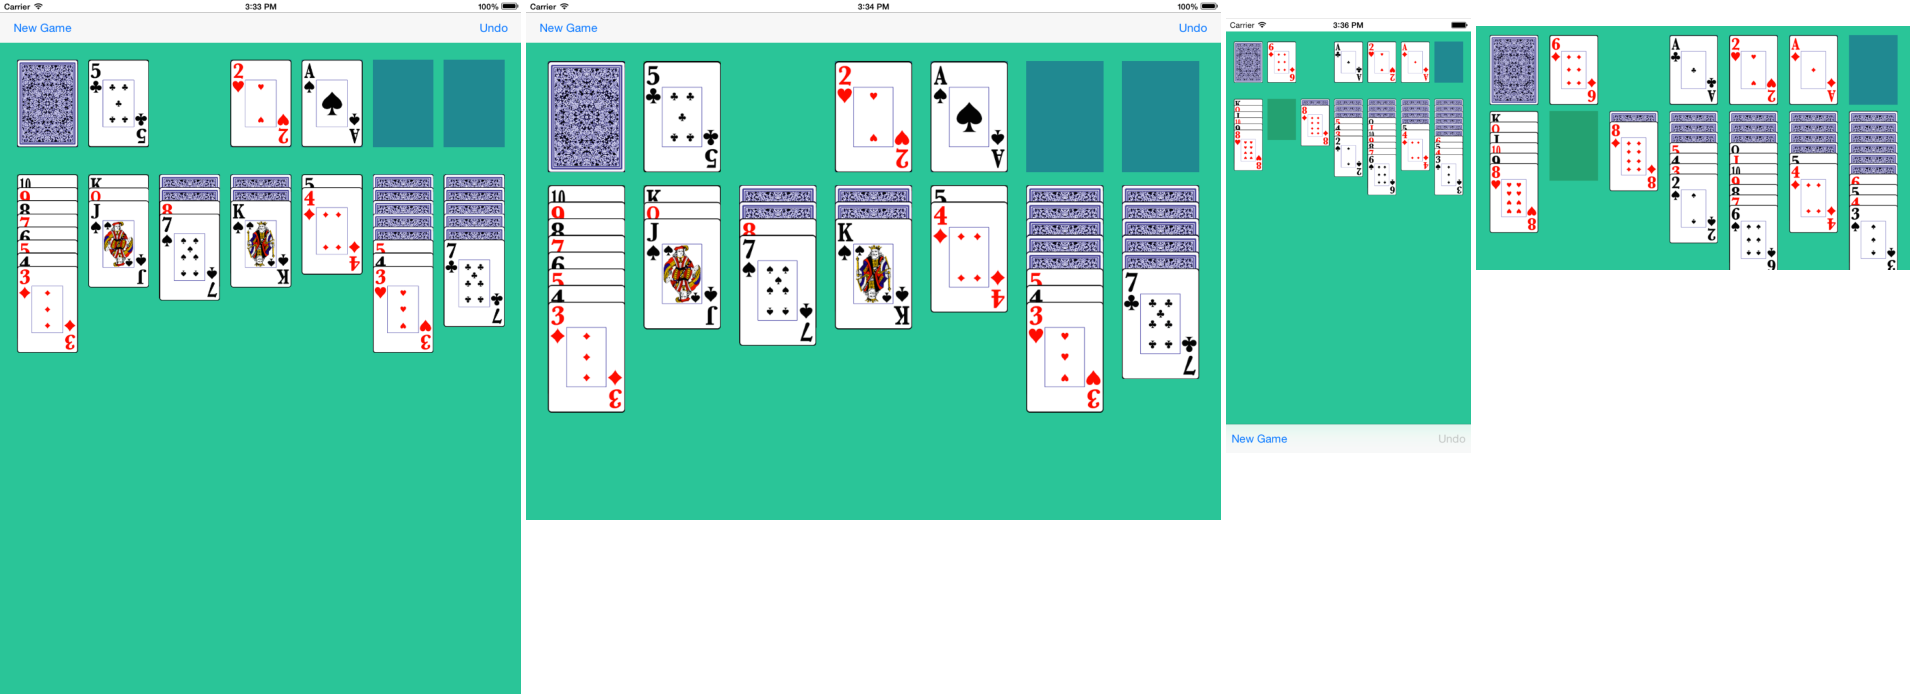
\includegraphics[width=\textwidth]{screenshots}
  \caption{Klondike Solitaire Screenshots on iPad~2 and iPhone~6.}
   \label{fig:screenshot}
\end{figure}

\section{Introduction}

This project describes an implementation of the popular 
{\em Klondike} solitaire card game for iOS.
For a detailed description of how its played check out wikipedia:
\begin{flushleft}
\url{http://en.wikipedia.org/wiki/Klondike_(solitaire)}
\end{flushleft}

%The game uses a standard 52-card deck of playing cards which
%are shuffled and dealt 
The game uses a standard 52-card deck of playing cards;
Each card is either face-up or face-down on a card table 
as illustrated in Figure~\ref{fig:screenshot}.
Section~\ref{sec:terms} explains the terminology for the
various regions of the card table. The MVC model elements represent
a deck of (immutable) playing cards and a game engine that records
the state of the game and dictates legal moves as
described in Section~\ref{sec:model}.
Section~\ref{sec:view} describes how to represent playing cards
and card table regions with Core Animation Layers.
Most of the user interaction is handled by the {\tt SolitaireView}
class in the implementation described here.
Other potential features are listed in Section~\ref{sec:bells-and-whistles}.

\pagebreak

\section{Card table terminology and layout} \label{sec:terms}

\begin{figure}[ht!] %  figure placement: here, top, bottom, or page
   \centering
   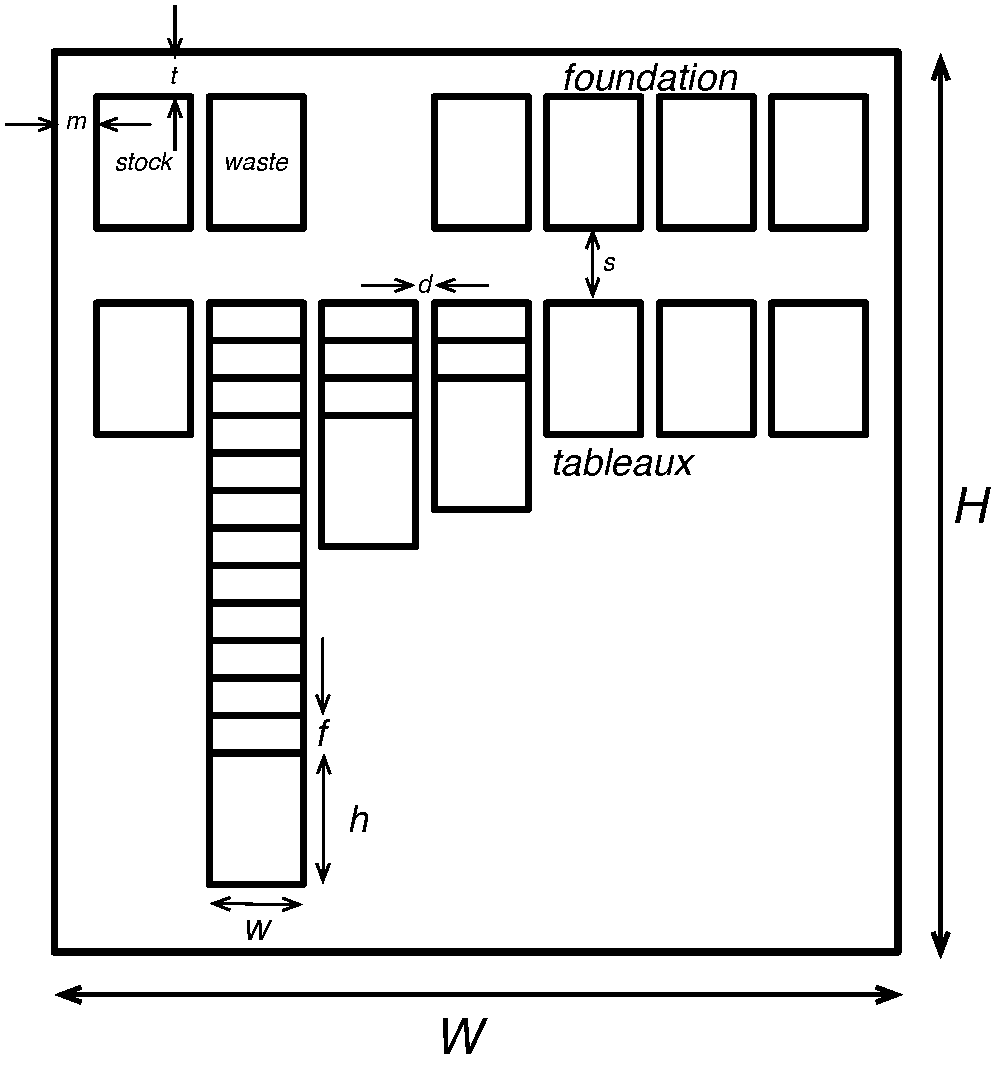
\includegraphics[width=0.5\textwidth]{card-table} 
   \caption{Layout of regions and cards.}
   \label{fig:card-table}
\end{figure}

There are thirteen regions that can hold stacks of cards
as illustrated in Figure~\ref{fig:card-table}:
\begin{description}
\item[stock] Holds cards (face down) not yet in play elsewhere.
  The user taps the top card to deal one or more cards (my app deals three)
  which are
  then flipped over and moved to the top of the waste.
\item[waste] Holds cards (face up) dealt from the stock. The user
  can move the top card onto one of the foundation or tableau stacks.
\item[foundation] One of four stacks that hold thirteen cards from ace to king
  all of the same suit. The goal is to get all 52 cards onto the foundation
  stacks.
\item[tableau] One of seven stacks that hold zero of more face down cards beneath
  a set of face up cards that alternate in color and descend in rank (ace is the
  lowest rank). A king may be placed on an empty tableau.
\end{description}



\section{The Model} \label{sec:model}

\subsection{Cards}

\begin{figure}[ht!]
\begin{center}
\begin{verbatim}
enum Suit : UInt8 {
    case SPADES = 0
    case CLUBS  = 1
    case DIAMONDS = 2
    case HEARTS = 3
}

let ACE   : UInt8 = 1
let JACK  : UInt8 = 11
let QUEEN : UInt8 = 12
let KING  : UInt8 = 13

func ==(left: Card, right: Card) -> Bool {
    return left.suit == right.suit && left.rank == right.rank
}

struct Card : Hashable {
    let suit : Suit  // .SPADES ... .HEARTS 
    let rank : UInt8 // 1 ... 13
    
    var hashValue: Int {
        return Int(suit.rawValue*13 + rank - 1) // perfect hash to 0 ... 51
    }
    
    init(suit s : Suit, rank r : UInt8) {
        suit = s;
        rank = r
    }
    ...
}
\end{verbatim}
\caption{We represent each playing card as an (immutable) {\tt struct} that encodes 
  the card's suit and rank. By conforming to the {\tt Hashable} protocol 
  we can use cards as dictionary keys.}
\label{fig:Card}
\end{center}
\end{figure}

We represent a playing card by its suit and rank as listed in Figure~\ref{fig:Card}.
The \verb@==@ operator is overloaded for {\tt Card}'s and we add a {\tt hashValue}
property so that {\tt Card}'s can be {\tt Hashable} (so we can use them as dictionary keys
and them in {\tt Set}'s.).

\subsection{Game Engine}

The state of the game and behaviors are defined  by a singleton object
(stored in the App Delegate) that is an instance of the {\tt Solitaire}
class which has the following interface:
\begin{description}
\item{\tt init()} Create new Solitaire game model object.
\item{\tt func freshGame()} Reshuffle and redeal cards to start a new game. 
\item{\tt func gameWon() -> Bool} All cards have successfully reached a foundation stack. 
%\item{\tt -(NSArray*)stock;}  Face down cards in stock.
%\item{\tt -(NSArray*)waste;} Face up card in waste.
%\item{\tt -(NSArray*)foundation:(int)i;} Cards on foundation $0 \leq i < 4.$ 
%\item{\tt -(NSArray*)tableau:(int)i;} Cards on tableau $0 \leq i < 7.$ 
\item{\verb@func isCardFaceUp(card : Card) -> Bool@} Is given card face up? 
\item{\verb@func fanBeginningWithCard(card : Card) -> [Card]?@} Array of face up
   cards found stacked on top of one of the tableau's. 
\item{\verb@func canDropCard(card : Card, onFoundation i : Int) -> Bool@}  Can the given
  cards be legally dropped on the $i$th foundation?
\item{\verb@func didDropCard(card : Card, onFoundation i : Int)@} The user did drop
  the given card on on the $i$th foundation.
\item{\verb@func canDropCard(card : Card, onTableau i : Int) -> Bool;@} Can the given card
  be legally dropped on the $i$th tableau?
\item{\verb@func didDropCard(card : Card, onTableau i : Int)@} The user did drop
  the card on the on the $i$th tableau.
\item{\verb@func canDropFan(cards : [Card], onTableau i : Int) -> Bool@} Can the given 
  stack of cards be legally dropped on the $i$ tableau?
\item{\verb@func didDropFan(cards : [Card], onTableau i : Int)@} A stack of
  cards has been dropped in the $i$th tableau.
\item{\verb@func canFlipCard(card : Card) -> Bool@} Can user legally flip the card over?
\item{\verb@func didFlipCard(card : Card)@} The user did flip the card over.
\item{\verb@func canDealCard() -> Bool@} Can user move top card from stock to waste?
\item{\verb@func didDealCard()@} Uses did move the top stack card to the waste.
\item{\verb@func collectWasteCardsIntoStock()@} Move all waste cards back to
  the stock (they're all flipped over -- order is maintained).
\end{description}
%My {\tt Solitaire} class conforms to the {\tt NSCoding} protocol so
%I can easily archive the state of the game in persistent store
%when the app is placed in the background:
%\begin{verbatim}
%@interface Solitaire : NSObject <NSCoding>
%...
%@end
%\end{verbatim}

\subsection{Internal representation}

Internally we store the various card stacks in arrays and keep track
of which cards are ``face up'' in a set:
\begin{verbatim}
class Solitaire {
    var stock : [Card]
    var waste : [Card]
    var foundation : [[Card]]  // Array of 4 card stacks
    var tableau : [[Card]]     // Array of 7 card stacks
    
    private var faceUpCards : Set<Card>;
    ...
}
@end
\end{verbatim}

\section{The View Elements} \label{sec:view}

\subsection{Displaying Poker Cards}

I represent each card visually using a custom
{\tt CALayer} subclass named {\tt CardLayer} -- each instance is permanently associated
with exactly one of the model's {\tt Card}s:
\begin{verbatim}
class CardLayer: CALayer {
    let card : Card
    var faceUp : Bool {
        didSet {
            if faceUp != oldValue {
                let image = faceUp ? frontImage : CardLayer.backImage
                self.contents = image?.CGImage
            }
        }
    }
    let frontImage : UIImage 
    static let backImage = UIImage(named: ...)
    
    init(card : Card) {
        self.card = card
        faceUp = true
        frontImage = imageForCard(card) // load associated image from main bundle
        super.init()
        self.contents = frontImage.CGImage
        self.contentsGravity = kCAGravityResizeAspect
    }
    ...
}
\end{verbatim}
%I set each {\tt CardLayer}'s {\tt contents} property to a {\tt CGImage}
%fetched from a set of PNG images stored in the app's bundle;
Each card image is stored in a {\tt UIImage} instance 
(loaded from PNG's stored the app's bundle at launch time)
whose {\tt CGImage} property is used to set the {\tt CardLayer}'s 
{\tt contents} property.
A single image is shared
by all {\tt CardLayer}'s to represent the backside of the card
and a unique image is used when the card is face up.
Using Core Animation layers has the advantage of being automatically
animated as they change position and their stacking order is
controlled by the {\tt zPosition} property. 

\subsection{The Card Table View}

Most of the UI interaction ({\it e.g.,} touching and dragging cards) 
is handled directly by my {\tt SolitaireView} class~\footnote{Perhaps it would
be more appropriate for the view controller to handle much of this logic.}
which encapsulates
the card table view elements and all the playing cards and has direct
access to the model object (lazy loaded from the App Delegate).
Internally I represent all the pertinent regions of the card
table with a {\tt CALayer} which are added (along with all 52 playing
cards) as sublayer's the view's main layer.
I use a dictionary to map a model {\tt Card} to its associated
{\tt CardLayer}. 
\begin{verbatim}
class SolitaireView: UIView {
    var stockLayer : CALayer!
    var wasteLayer : CALayer!
    var foundationLayers : [CALayer]!  // four foundation layers
    var tableauLayers : [CALayer]!     // seven tableau layers
    
    var topZPosition : CGFloat = 0  // "highest" z-value of all card layers
    var cardToLayerDictionary : [Card : CardLayer]! // map card to it's layer
    
    var draggingCardLayer : CardLayer? = nil // card layer dragged (nil => no drag)
    var draggingFan : [Card]? = nil          // fan of cards dragged
    var touchStartPoint : CGPoint = CGPointZero
    var touchStartLayerPosition : CGPoint = CGPointZero
    
    lazy var solitaire : Solitaire!  = { // reference to model in app delegate
        let appDelegate = UIApplication.sharedApplication().delegate as! AppDelegate
        return appDelegate.solitaire
    }()
    ...
 }
@end
\end{verbatim}

\subsubsection{Initializing the View}

An instance of my {\tt SolitaireView}, which is stored in the StoryBoard, is
further initialized after it has been deserialized from the StoryBoard.
Each layer is created and added as a sublayer to the view's main layer.
Each layer is given a name for future identification on user touches.
\begin{verbatim}
override func awakeFromNib() {
    self.layer.name = "background"
      
    stockLayer = CALayer()
    stockLayer.name = "stock"
    stockLayer.backgroundColor = 
        UIColor(colorLiteralRed: 0.0, green: 0.5, blue: 0.0, alpha: 0.3).CGColor
    self.layer.addSublayer(stockLayer)
    
    ... create and add waste, foundation, and tableau sublayers ...
    
    let deck = Card.deck() // deck of poker cards
    cardToLayerDictionary = [:]
    for card in deck {
        let cardLayer = CardLayer(card: card)
        cardLayer.name = "card"
        self.layer.addSublayer(cardLayer)
        cardToLayerDictionary[card] = cardLayer
    }
 }
\end{verbatim}
The actual positions and sizes of each layer is determined later
as described in the next section.

\subsubsection{Table Layout}

The various sublayers are (re)arranged when the orientation
of the app changes which triggers the 
view's {\tt layoutSublayersOfLayer:} method:
\begin{verbatim}
override func layoutSublayersOfLayer(layer: CALayer) {
    draggingCardLayer = nil // deactivate any dragging
    layoutTableAndCards()
}
\end{verbatim}
%The controller determines when the orientation of the app changes
%and requests that the table layout its sublayers appropriately.
The view provides a method that determines the size and position
of each layer based on the current view geometry:
\begin{verbatim}
func layoutTableAndCards() {
    let width = bounds.size.width
    let height = bounds.size.height
    let portrait = width < height
    
    ... determine size and position of stock, waste, foundation
         and tableau layers ...
    
    layoutCards()
}
\end{verbatim}
The size, position, and z-order of each card layer is computed
in the method below. The cards in each tableau stack is fanned downwards.
\begin{verbatim}
func layoutCards() {
    var z : CGFloat = 1.0
      
    let stock = solitaire.stock
    for card in stock {
        let cardLayer = cardToLayerDictionary[card]!
        cardLayer.frame = stockLayer.frame
        cardLayer.faceUp = solitaire.isCardFaceUp(card)
        cardLayer.zPosition = z++
    }
 
    ... layout cards in waste and foundation stacks ...
    
    let cardSize = stockLayer.bounds.size
    let fanOffset = FAN_OFFSET * cardSize.height
    for i in 0 ..< 7 {
        let tableau = solitaire.tableau[i]
        let tableauOrigin = tableauLayers[i].frame.origin
        var j : CGFloat = 0
        for card in tableau {
            let cardLayer = cardToLayerDictionary[card]!
            cardLayer.frame = 
                CGRectMake(tableauOrigin.x, tableauOrigin.y + j*fanOffset, 
                           cardSize.width, cardSize.height)
            cardLayer.faceUp = solitaire.isCardFaceUp(card)
            cardLayer.zPosition = z++
            j++
        }
    }
    
    topZPosition = z  // remember "highest position"
}
\end{verbatim}


\subsubsection{Dragging and Tapping Cards}

Most of the user interaction involves the user selecting a card (or stack
of cards), dragging them to another location, and dropping them on
a stack. Other gestures can trigger actions as well:
\begin{enumerate}
\item The user taps on the top card of the stock when wanting to
  ``deal'' another card;
\item A tap on the stock causes all the waste cards to be collected
  back into the stock;
\item A double tap provides a shortcut that automatically moves a
  top face-up card to a foundation stack (if legal).
\end{enumerate}
Most actions begin on a user touch where we can use 
{\tt CALayer}'s {\tt hitTest:} method to determine which layer was touched:
\begin{verbatim}
override func touchesBegan(touches: Set<UITouch>, withEvent event: UIEvent?) {
    let touch = touches.first!
    let touchPoint = touch.locationInView(self)
    let hitTestPoint = self.layer.convertPoint(touchPoint, toLayer: self.layer.superlayer)
    let layer = self.layer.hitTest(hitTestPoint)
        
    if let layer = layer {
        if layer.name == "card" {
            let cardLayer = layer as! CardLayer
            let card = cardLayer.card
            if solitaire.isCardFaceUp(card) {
                ...if tap count > 1 move to foundation if allowed...
                ...else initiate drag of card (or stack of cards) by setting
                   draggingCardLayer, and (possibly) draggingFan...
            } else if solitaire.canFlipCard(card) {
                flipCard(card, faceUp: true) // update model & view
            } else if solitaire.stock.last == card {
                dealCardsFromStockToWaste();
            } 
        } else if (layer.name == "stock") {
             collectWasteCardsIntoStock()
        }
    }
}
\end{verbatim}
The following method is used to drag or move a {\tt CardLayer} (or a fanned stack of
{\tt CardLayer's}). The instance variables
{\tt draggingCardLayer} and {\tt draggingFan} are set
in the {\tt touchesBegan:withEvent:} method when the user selects
a card (or stack of cards) to drag.
While the user is dragging cards 
({\it e.g.,} while processing a \verb@touchesMoved:withEvent:@ message)
we want to disable animation, 
but otherwise we animate the change of position:
\begin{verbatim}
func dragCardsToPosition(position : CGPoint, animate : Bool) {
    if !animate {
        CATransaction.begin()
        CATransaction.setDisableActions(true)
    }
    draggingCardLayer!.position = position
    if let draggingFan = draggingFan {
        let off = FAN_OFFSET*draggingCardLayer!.bounds.size.height
        let n = draggingFan.count
        for i in 1 ..< n {
            let card = draggingFan[i]
            let cardLayer = cardToLayerDictionary[card]!
            cardLayer.position = CGPointMake(position.x, position.y + CGFloat(i)*off)
        }
    }
    if !animate {
        CATransaction.commit()
    }
}
\end{verbatim}
For example, if the user drops a fan of cards in a bogus location, we can
use this method to animate moving them back to their original position.

\subsubsection{Dropping Card(s)}

When a touch sequence ends we need to do the following:
\begin{enumerate}
\item Determine where the user is attempting to drop
  the card(s) by comparing the frame of
  the layer being dragged with all the frames of potential target layers
  (\verb@CGRectIntersectsRect@ is useful here).
\item Check to see if this is a valid drop (can't just drop them anywhere) 
  and a legal drop (consult the model).
\item If the drop is okay, then the model needs to be informed of the change
  and the view needs to updated accordingly.
\item If the drop is {\em not} okay, then the card(s) need to moved back
\end{enumerate}
\begin{verbatim}
override func touchesEnded(touches: Set<UITouch>, withEvent event: UIEvent?) {
    if let dragLayer = draggingCardLayer {
       if dragging only one card {
          ... determine where the user is trying to drop the card
          ... determine if this is a valid/legal drop
             ... if so, update model and view
             ... else put card back from whence it came
       } else { // fan of cards (can only drop on tableau stack)
          ... determine if valid/legal drop
            ... if so, update model and view
            ... else put cards back from whence they came
       }
       draggingCardLayer = nil
    }
}
\end{verbatim}

\section{Other Bells and Whistles} \label{sec:bells-and-whistles}

\subsection{Persistent Store}

When the app enters the background, the state of the model should
be saved in the app's sandbox. 
Note that my {\tt Card} type is a Swift {\tt struct} (not a {\tt class})
and thus can not conform to the {\tt NSCoding} protocol for archival purposes.
Instead I allow {\tt Card}'s to be created/saved from/to a {\em property
list} (plist) compatible dictionary:
\begin{verbatim}
struct Card : Hashable {
    let suit : Suit
    let rank : UInt8 // 1 .. 13
    ...
    init(dictionary dict : [String : AnyObject]) { // to retrieve from plist
        suit = Suit(rawValue: (dict["suit"] as! NSNumber).unsignedCharValue)!
        rank = (dict["rank"] as! NSNumber).unsignedCharValue
    }
    
    func toDictionary() -> [String : AnyObject] { // to store in plist
        return [
            "suit" : NSNumber(unsignedChar: suit.rawValue),
            "rank" : NSNumber(unsignedChar: rank)
        ]
    }
    ...    
 }   
\end{verbatim}
Similarly I allow my {\tt Solitaire} model class to be persistently stored
as a plist:
\begin{verbatim}
class Solitaire {
    var stock : [Card]
    var waste : [Card]
    var foundation : [[Card]]
    var tableau : [[Card]]
    private var faceUpCards : Set<Card>;
    ...
    init(dictionary dict : [String : AnyObject]) { // for retrieving from plist
       ...
    }
    
    func toDictionary() -> [String : AnyObject] {  // for storing in plist
       ...
    }
}
\end{verbatim}
When the app enters the background state, save the game's state
as a plist in the app's sandbox.
When the app is launched, check to see if the state of the
previous run has been saved; If so, load the model state from
the plist stored in the app's sandbox,
otherwise create a new (random) game.

\subsection{Animating the deal}

If you are dealing more than one card at a time when 
the use touches the card on the top of the stock, there
should be a sequence of animations triggered
for each card. Don't forget to update the layer's model
layer before each animation so that the final resting
place each dealt card persists!

\subsection{Undo}

%Having one level of undo is a nice feature (more than this tempts
%the user to cheat). 
Allowing the user to undo (and redo) actions is a nice feature (but
maybe encourages cheating).
To accomplish this you need to
record the appropriate set of actions that undo (and redo) the
recent actions. You might not realize it, but your app already has
an {\tt undoManager} property that is an instance of
{\tt NSUndoManager} that handles a lot of this machinery.
In fact, it is already wired to respond to a shake gesture if you
make your view a first responder.
Recording all the necessary actions is a bit of work -- see your textbook
on undo manager (or come talk to me) if you are really interested.

\subsection{Party when the user wins!}

The user should get some sort of visual ``pay off'' when
(s)he wins. A cool card animation might be the ticket.

\subsection{Finishing up}

Polishing the final app and following the steps needed
for submission to the iTune's store is worth practicing.
This can easily be made into a universal app that operates
in all orientations -- the trick
is making the cards just the right size and placing the
tableaus so you can see up to $6 + 13$ cards fanned out
(6 face-down cards plus king through ace).


\end{document}  